\begin{center}
    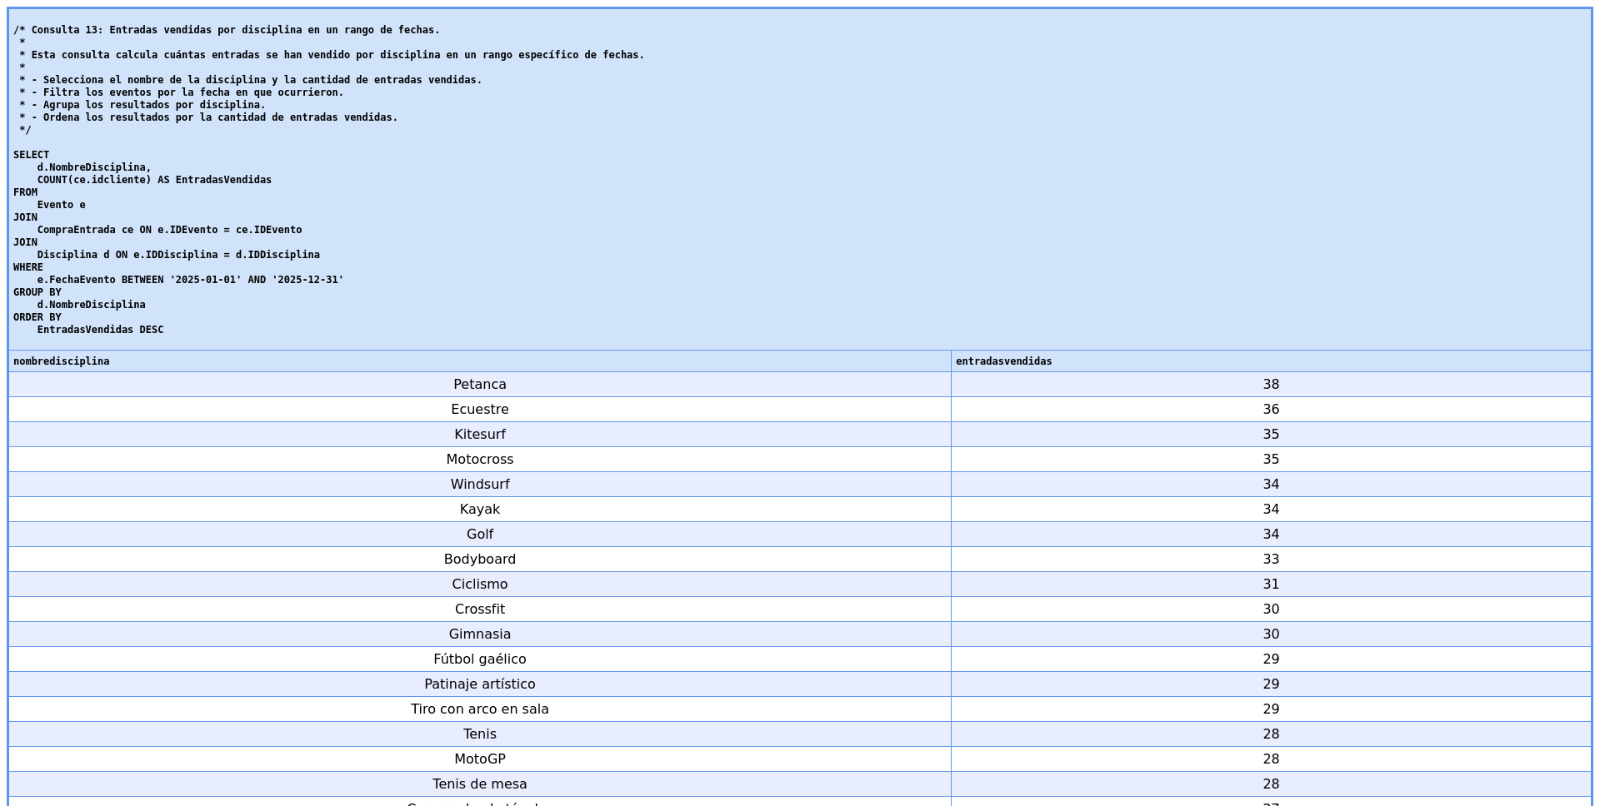
\includegraphics[width=16.5cm]{resources/Consulta13.jpeg} 
    
   Consulta 13. Entradas vendidas por disciplina en un rango de fechas.
\end{center}

\textbf{Propósito de la consulta}

El objetivo de esta consulta es determinar la cantidad de entradas vendidas por disciplina durante un rango específico de fechas. Esto permite analizar la popularidad de las disciplinas y apoyar la toma de decisiones en la planificación de futuros eventos.

\textbf{Desglose de la consulta}

\begin{itemize}
   \item \textbf{Selección de columnas (\texttt{SELECT})}:
   \begin{itemize}
       \item \texttt{d.NombreDisciplina}: Nombre de la disciplina deportiva.
       \item \texttt{COUNT(ce.IDCliente)}: Calcula la cantidad de entradas vendidas para cada disciplina. Esta columna se denomina \texttt{EntradasVendidas}.
   \end{itemize}

   \item \textbf{Tablas involucradas (\texttt{FROM} y \texttt{JOIN})}:
   \begin{itemize}
       \item \texttt{Evento (e)}: Contiene información sobre los eventos deportivos.
       \item \texttt{CompraEntrada (ce)}: Contiene información sobre las compras de entradas.
       \item \texttt{Disciplina (d)}: Contiene información sobre las disciplinas deportivas.
       \item Se realizan los siguientes \texttt{JOINs}:
       \begin{itemize}
           \item \texttt{Evento} con \texttt{CompraEntrada} usando \texttt{e.IDEvento = ce.IDEvento}, para relacionar las entradas con los eventos.
           \item \texttt{Evento} con \texttt{Disciplina} usando \texttt{e.IDDisciplina = d.IDDisciplina}, para asociar los eventos con las disciplinas correspondientes.
       \end{itemize}
   \end{itemize}

   \item \textbf{Filtrado de datos (\texttt{WHERE})}:
   \begin{itemize}
       \item Se filtran los eventos cuya fecha (\texttt{e.FechaEvento}) esté dentro del rango especificado: entre el 1 de enero y el 31 de diciembre de 2025.
   \end{itemize}

   \item \textbf{Agrupación de resultados (\texttt{GROUP BY})}:
   \begin{itemize}
       \item Los resultados se agrupan por \texttt{d.NombreDisciplina}, para calcular la cantidad total de entradas vendidas por cada disciplina.
   \end{itemize}

   \item \textbf{Ordenamiento de resultados (\texttt{ORDER BY})}:
   \begin{itemize}
       \item Los resultados se ordenan en orden descendente (\texttt{DESC}) según la cantidad de entradas vendidas (\texttt{EntradasVendidas}), mostrando primero las disciplinas más populares.
   \end{itemize}
\end{itemize}

\textbf{Análisis detallado}

\begin{enumerate}
   \item \textbf{Relación entre tablas:}
   \begin{itemize}
       \item Existe una relación entre las tablas \texttt{Evento}, \texttt{CompraEntrada} y \texttt{Disciplina}:
       \begin{itemize}
           \item Cada entrada comprada se asocia con un evento a través de \texttt{IDEvento}.
           \item Cada evento está vinculado a una disciplina mediante \texttt{IDDisciplina}.
       \end{itemize}
   \end{itemize}
   
   \item \textbf{Cálculo de entradas vendidas:}
   \begin{itemize}
       \item La función agregada \texttt{COUNT(ce.IDCliente)} cuenta el número de entradas vendidas asociadas con cada disciplina.
   \end{itemize}
   
   \item \textbf{Filtrado por rango de fechas:}
   \begin{itemize}
       \item El filtro en el \texttt{WHERE} asegura que solo se incluyan eventos ocurridos en 2025, excluyendo datos fuera de este rango temporal.
   \end{itemize}
   
   \item \textbf{Ordenamiento:}
   \begin{itemize}
       \item Ordenar por \texttt{EntradasVendidas DESC} permite identificar las disciplinas con mayor éxito en ventas de entradas.
   \end{itemize}
\end{enumerate}

\textbf{Consideraciones}

\begin{itemize}
   \item \textbf{Eventos sin ventas:}
   \begin{itemize}
       \item Si una disciplina no tuvo ventas de entradas, no aparecerá en los resultados.
   \end{itemize}
   \item \textbf{Empates en las ventas:}
   \begin{itemize}
       \item Si dos disciplinas tienen la misma cantidad de entradas vendidas, el orden relativo entre ellas no está definido. Se podría agregar un criterio adicional en el \texttt{ORDER BY}, como el nombre de la disciplina.
   \end{itemize}
\end{itemize}

\textbf{Utilidad de la consulta}

Esta consulta es útil para:
\begin{itemize}
    \item Evaluar la popularidad de las disciplinas en función de las ventas de entradas.
    \item Identificar disciplinas que podrían necesitar estrategias de promoción o mejor planificación logística.
    \item Ayudar en la asignación de recursos y espacios para futuras competencias basadas en la demanda histórica.
    \item Determinar patrones de participación del público durante un rango de fechas específico.
\end{itemize}
